\chapter{Observações do Estudo}

Durante este capítulo, será apresentada uma introdução sobre o ambiente de trabalho e a plataforma de desenvolvimento, chamada Noosfero. A partir desta introdução apresentaremos os a avaliação de usabildiade, assim como os testes e as funcionalidades desenvolvidas dentro do processo de colaboração com esta plataforma.

\section{Estudo de Caso - Noosfero}

Noosfero\footnote{\url{noosfero.org}} é uma plataforma desenvolvida pela Colivre (Cooperativa de Tecnologias Livre)\footnote{url{colivre.coop.br}}, possui licença AGPL e é utilizado, principalmente em universidades públicas, para desenvolvimento de redes colaborativas. \footnote{url{http://softwarelivre.org/colivre/blog/projeto-noosfero}}
%
O noosfero foi desenvolvido na linguagem de programação Ruby, versão 1.8.7, e utiliza
o framework Model-View-Controller (MVC) para aplicações web Ruby on Rails, versão 
2.3.5. A escolha destas tecnologias, por parte dos criadores do Noosfero foi baseada 
fato de que o Ruby possui sintaxe simples, elegante e de fácil leitura, o que aumenta
a manutenibilidade do sistema, uma característica importante num projeto de software
livre que visa atrair desenvolvedores externos~\cite{meirelles2013}.

\subsection{Desenvolvimento no processo de colaboração ao noosfero}

Por tratar de um software livre, a plataforma Noosfero possui uma grande quantidade 
de colaboradores, formado por equipes de desenvolvimento como na Universidade de 
Brasília, ou por desenvolvedores independentes. Assim, para que haja sucesso na 
colaboração, são feitas exigências durante o desenvolvimento, assim como testes 
bem definidos para aprovar novas funcionalidade.

Além da utilização da linguagem de programação \textit{Ruby}, o desenvolvimento da plataforma noosfero também se baseia em JavaScript, CSS, dentre outras linguagens, como pode-se ver na figura abaixo:
%
\begin{figure}[!h]
    \centering
    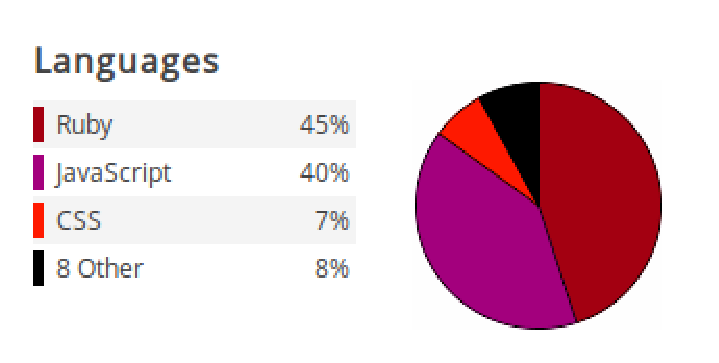
\includegraphics[keepaspectratio=true,scale=0.60]
      {figuras/noosfero.eps}
    \caption{Desenvolvimento noosfero}
    \label{noosfero}
\end{figure}

O desenvolvimento para a plataforma Noosfero é realizado em ciclos e, pela Colivre, 
possui as seguintes fases: desenvolvimento, release 1, release 2 e release final.

\subsubsection{Fase de Desenvolvimento}
%
Antes da fase de desenvolvimento for iniciada é necessário que seja feita a 
documentação do que será desenvolvido. Os desenvolvedores responsáveis criam um 
\textit{action item} (item de ação), contendo a história de usuário ou os requisitos do novo 
recurso. Um \textit{action item} pode ser descrito como uma \textit{feature} (novo recurso) ou como 
um \textit{bug} (defeito) encontrado, como demonstrado nas figuras abaixo:\footnote{url{noosfero.org}}
%
\begin{figure}[!h]
    \centering
    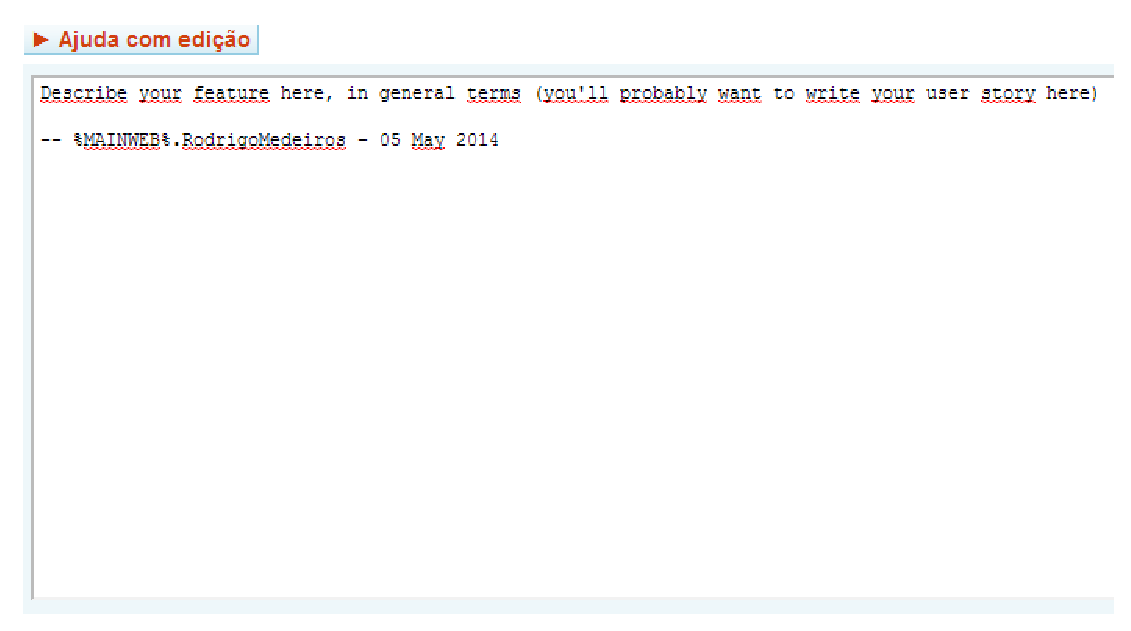
\includegraphics[keepaspectratio=true,scale=0.65]
      {figuras/noosfero_feature.eps}
    \caption{Descrição de \textit{feature} - noosfero}
    \label{noosfero_feature}
\end{figure}
%
\begin{figure}[!h]
    \centering
    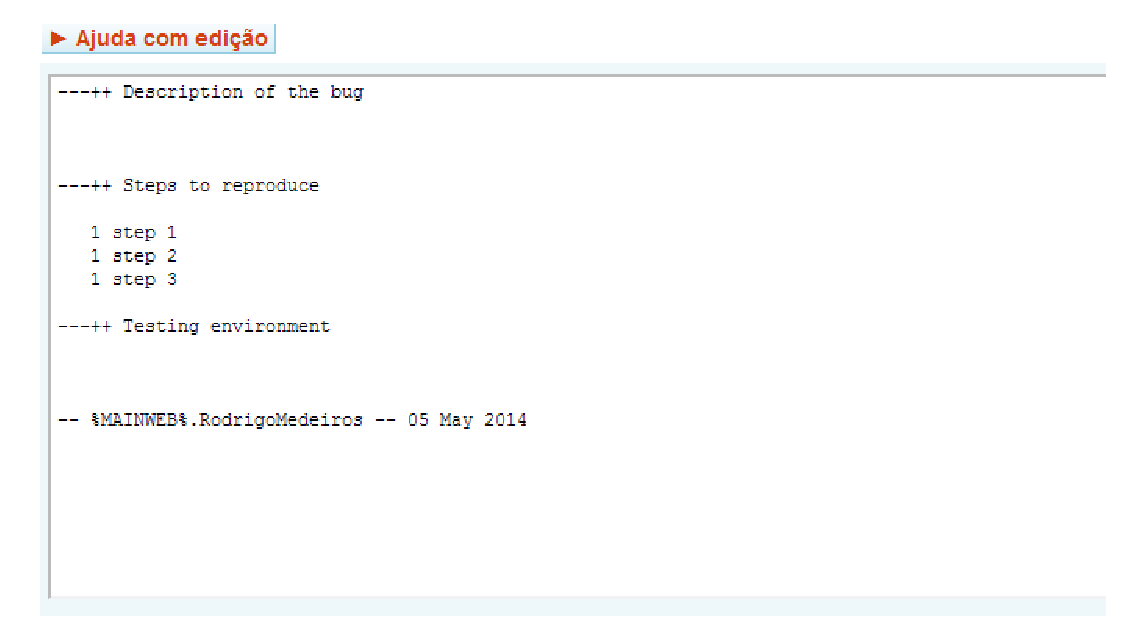
\includegraphics[keepaspectratio=true,scale=0.65]
      {figuras/noosfero_bug.eps}
    \caption{Descrição de \textit{bug} - noosfero}
    \label{noosfero_bug}
\end{figure}

%------------------------------------------------------------------------------%

Além da documentação, é necessário o envio de um \textit{email} a comunidade descrevendo o 
que será desenvolvido. A partir deste \textit{email}, a comunidade irá avaliar a funcionalidade 
descrita e decidir se é um funcionalidade importante para se incorporar ou não. 
Este processo de avaliação tem a duração de uma semana, geralmente.\footnote{url{noosfero.org}}

Com a aprovação da comunidade são feitas as revisões do ciclo de desenvolvimento, 
que deve seguir os seguintes passos:
%
\begin{enumerate}
\item Criar um \textit{‘merge request’} juntamente com o código;
\item Código é revisado pela comunidade;
\item Código é bom? 
\subitem Se sim:
\subsubitem Vá para o passo 4;
\subitem Se não:
\subsubitem \textit{‘Merge request’} é rejeitado e as razões por tal são comentadas e 
respondidas;
\subsubitem Desenvolvedores revisam o que está errado;
\item Código é incluido no código principal.
\end{enumerate}
%------------------------------------------------------------------------------%
\subsubsection{Fase de Release 1}
%
A entrega da \textit{release} consiste na instalação da nova versão do código no repositório de testes, assim como no código principal quando não houver mais defeitos, ou todos os defeitos encontrados forem tratados devidamente. Porém se algum erro crítico for encontrado e não for tratado a tempo da \textit{release} final, o lançamento pode ser adiado para a próxima \textit{release}.
%
\subsubsection{Fase de Release 2}
%
A \textit{release} 2 não é obrigatória, so ocorre se houver muitas mudanças na \textit{release} 1 e requerer novos testes. Vale lembrar que os procedimentos realizados para aprovar a \textit{release} 2 são os mesmos da \textit{release} 1%Referenciar%
%
\subsubsection{Release Final}
%
A versão final do código é lançada após todos os testes serem aprovados nas \textit{releases} 1 e 2, assim o código pode ser atualizado para o código principal do noosfero, encerrando o ciclo de desenvolvimento.\footnote{\url{noosfero.org}}

\subsection {Aplicações}

O estudo deste trabalho é baseado em duas aplicações que utilizam a plataforma noosfero, o portal Participa Br e o Comunidade UnB.

O Portal da participação Social é um portal que agrega informações sobre oportunidades de participação social no governo federal e estimula a formação de comunidades em torno de temas ligados à participação. Informa sobre as consultas públicas, oferece ambientes para interação em vídeo e chat em eventos de governo. É um repositório das metodologias das conferências de políticas públicas. O Portal capta demandas da sociedade que não passem, necessariamente, pelos fluxos formais de participação. É uma plataforma para ampliar o debate entre a sociedade civil e o governo. [Citar fonte]

A rede Comunidade UnB, que se encontra em ambiente de testes, porém disponível para acesso externo, contando com aproximadamente 160 usuários ativos. A rede Comunidade UnB é uma instância do noosfero instalada através de um pacote em um servidor do Centro de Difusão de Tecnologia e Conhecimetno (CDTC)\footnote{\url{www.cdtc.org.br}} da UnB. O propósito da rede Comunidade UnB é tornar-se um ambiente de colaboração entre os alunos da Universidade de Brasília, tanto de graduação quanto de pós-graduação, possibilitando criação comunidades e blogs para discussões, ou a disponibilização de artigos, trabalhos de graduação e pós-graduação onde qualquer membro da universidade tenha acesso.

\section {Estudo sobre Usabilidade - Portal da Participação Social}

\subsection{Introdução}

O Portal da Participação Social \footnote{\url{participa.br}} é um portal que agrega informações sobre oportunidades de participação social no governo federal e estimula a formação de comunidades em torno de temas ligados à participação. Informa sobre as consultas públicas, oferece ambientes para interação em vídeo e chat em eventos de governo. É um repositório das metodologias das conferências de políticas públicas. O Portal capta demandas da sociedade que não passem, necessariamente, pelos fluxos formais de participação. É uma plataforma para ampliar o debate entre a sociedade civil e o governo. % [Citar fonte]

\subsection{Justificativa}	

	A ideia de fazer esses estudo experimental era de conhecer e aplicar as técnicas existentes na engenharia de usabilidade em um contexto real de uso para verificar como funcionam as técnicas utilizadas na engenharia de usabilidade para avaliação de um website.
	
		

	% verificar essa justificativa

	No ano 2000 foi criado o programa de Governo Eletrônico (e-GOV) \footnote{\url{www.governoeletronico.gov.br}} que têm como principais objetivos democratizar o acesso a informação e dinamizar a prestação de serviços públicos eletrônicos com foco em eficiência e efetividade das funções governamentais prestadas ao cidadão.

	O Governo Federal adotou várias práticas de padrões para melhorar o acesso e a divulgação das informações e dos serviços do governo eletrônico, respeitando as particularidades de cada cidadão. Por isso foi criado o Modelo de Acessibilidade do Governo Federal (e-MAG) \footnote{e-MAG <portal>} que contém um conjunto de recomendações para tornar os sítios e portais acessíveis para uma maior quantidade de pessoas possíveis. 

	O objetivo era de estabelecer padrões de qualidade de uso, desenho, arquitetura da informação e navegação, desenvolvimento e manutenção na gestão dos sítios governamentais.O  e-PWG \footnote{e-PWG <portal>}, como ficou conhecido, são padrões web para o Governo eletrônico.

	Foi feita uma análise do sítio participa.br em parceria com o Instituto Federal do Rio Grande do Sul (IFRS) onde foi criado um relatório para orientar e sugerir correções que facilitarão o acesso ao seu conteúdo quanto as recomendações sobre o Modelo de Acessibilidade em Governo Eletrônico (e-MAG) e com os Padrões Web em governo Eletrônico (e-PWG). Essas recomendações busca levantar problemas que impactarão na experiência de uso do portal pelo cidadão.

	Como já existia um estudo referente sobre a Acessibilidade do portal participa.br o nosso estudo se deu em avaliar a qualidade em uso do portal no sentido de verificar a satifação dos usuários ao utilizar o portal.

	Primeiramente foi preciso realizar um checklist de usabilidade para verificar os possíveis problemas no portal antes de realizar os testes com os usuários.Foi utilizado as heurísticas de Nielsen para identificação dos problemas de usabilidade.

\subsection{Definição do Estudo Experimental}

\subsubsection{Objetivo Global}

	Analisar a interação dos usuários com o portal participa.br a fim de avaliar a qualidade em uso dos usuários com este portal. 

\subsubsection{Objetivos de Medição}

\begin{itemize}
\item Conhecer quem são os usuários do Portal da Participação Social.
\item Verificar problemas de usabilidade no Portal da Participação Social
\item Avaliar de forma subjetiva o grau de satisfação dos usuários com a utilização do portal participa.br. 
\end{itemize}


\subsubsection{Objetivo do Estudo}


\begin{table}[h]
\begin{tabular}{|l|l|}
\hline
Analisar             & Portal da Participação Social (participa.br) \\ \hline
Com propósito de     & Avaliar Qualidade em Uso (ISO/IEC 9126-4)    \\ \hline
Com respeito ao      & Satisfação do usuário                        \\ \hline
Do ponto de vista de & Usuário                                      \\ \hline
No contexto de       & Portais Governamentais                       \\ \hline
\end{tabular}
\caption {Objetivos do Estudo}
\end{table}

\subsubsection{Questões}

A partir do objetivo de medição estabelecido no quadro 1  foram definidas questões sobre o que é preciso saber de forma a apoiá-la a entender se o objetivo específico foi alcançado, e para cada questão foram definidas as métricas relacionadas no quadro 2: 

\begin{table}[h]
\begin{tabular}{|l|l|l|}
\hline
\textbf{Questões}  & Métricas    & \begin{tabular}[c]{@{}l@{}}Diretrizes para \\ interpretação \end{tabular}  \\ \hline
\begin{tabular}[c]{@{}l@{}} Q1. Qual o perfil do usuário \\ que utiliza o portal participa.br?  \end{tabular} &                Perfil               & \begin{tabular}[c]{@{}l@{}} Análise de Dados Estatísticos,\\ criação de personas, análise \\ dos dados qualitativos. \end{tabular}\\ \hline
\begin{tabular}[c]{@{}l@{}} Q2. Qual o grau de satisfação\\ do usuário que utiliza o portal \\ participa.br \end{tabular} &  \begin{tabular}[c]{@{}l@{}} Grau de satisfação \\ do usuário \end{tabular} & \begin{tabular}[c]{@{}l@{}} Escore da satisfação global\\ pelo usuário (OVERALL)   \end{tabular}                               \\ \hline
\begin{tabular}[c]{@{}l@{}} Q3. Quantidade de tempo gasto \\ para realizar as tarefas   \end{tabular}   &            Duração                   & Tempo gasto                       \\ \hline
\end{tabular}
\caption{Questões de Pesquisa}
\end{table}

\subsection{Metodologia}

\subsubsection{Análise do Perfil dos Usuários}

	Foram levantadas algumas técnicas na qual podemos identificar o perfil dos usuários do portal da Participação Social.
\begin{enumerate}
\item \textbf{Dados Estatísticos} (Google analytcs, piwiki, entre outros): Através dos dados estatisticos é possivel identificar algumas informações sobre o perfil dos usuários que acessam o portal. Nas pesquisas quantitativas não são necessários o contato direto com o usuário. Esses dados estatísticos podem ser coletados de base de dados, redes sociais ou sistemas de análises de sites.

\item \textbf{Questionário de identificação de perfil dos usuários:} Para identificar o perfil dos usuários do Portal da Participação social é necessário realizar uma pesquisa qualitativa para levantamento das principais caracterísiticas contextuais dos usuários típicos, de modo a comprender quem são, qual o conhecimento e experiência com a internet e como utilizam para realizar seu trabalho acadêmico ou profissional. A realização dessa pesquisa será feita com os usuários do Portal da Participação Social \footnote{\url{participa.br}}

A análise do questionário servirá para entender o perfil de usuários do Portal da participação social, através da investigação de seus interesses.Foi levantado também algumas questões referentes ao uso das funcionalidades do portal da participação social.


\item \textbf{Identificação de Personas:} Para a definição de usuários podemos utilizar a técnica de “Persona” que são personagens fícticios criados com base em dados reais. Os Personas atuam como representantes dos usuários reais e representam as necessidades de um grupo maior. 

	A utilização de Personas permite ter um maior foco no usuário, deixando o projeto centrado no usuário. É utilizado para a identificação de requisitos, criação de cenários e \textit{user stories}. 

	Para podermos identificar os personas primeiramente temos que realizar uma pesquisa quantitativa no qual podemos identificar os grupos de usuários. Após a identificação dos grupos de usuários é realizado a pesquisa qualitativa (entrevistas, coleta de dados) na qual podemos identificar as necessidades dos usuários de um determinado portal.

	Para criação do persona será necessário realizar entrevista com 3 pessoas de cada grupo alvo (universitários, ativistas políticos, servidores públicos, etc).

\end{enumerate}

\subsubsection{Paradigma e Técnica de Avaliação}

As medidas de usabilidade do sistema foram obtidas considerando-se três fatores: eficácia, eficiência e satifação de uso.

Neste experimento foi adotado como paradigma de avaliação o Teste de Usabilidade que consiste em avaliar o desempenho dos usuários na execução de tarefas cuidadosamente preparadas, tarefas estas dentro do escopo do sistema. Esse desempenho pode ser avaliado no quesito, número de erros e tempo de execução da tarefa.

A avaliação da usabilidade coletará tantos dados subjetivos em um cenário real como dados objetivos. Os dados subjetivos serão coletados através de opiniões dos participantes, comentários em relação ao uso do portal da participação social. Os dados objtivos consistem em medidas de tempo e desempenho dos participantes.

Para avaliar a usabilidade do portal participa.br serão utilizadas as técnicas:

\begin{table}[h]
\begin{tabular}{|l| p{10cm} |}
\hline
Técnica & Descrição \\ \hline
Observar Usuários & Um observador irá registrar o tempo 
gasto por cada participante para concluir o estudo de caso, 
avaliar a ferramenta e se necessitou de alguma ajuda    \\ \hline
Perguntar aos usuários & Os questionários ASQ e PSSUQ 
de satisfação dos usuários será utilizado 
para coletar as opiniões dos participantes.\\ \hline
\end{tabular}
\caption{Técnicas de avaliação para os testes com usuários}
\end{table}

\subsubsection{Heurísticas de Usabilidade}

	Segundo as pesquisa realizadas é necessário que antes que execute um teste de usabilidade seja feito uma avaliação da usabilidade por parte de especialistas de usabilidade. Através das heurísticas de Nielsen identificamos os problemas inerentes ao portal da participação social.

\subsubsection{Instrumentos para coletas de dados}

	Os intrumentos de coletas de informações utilizados são dois questionários que são amplamentes utilizados para medir a satisfação do usuário com produtos interativos e fornecem medidas padronizadas. São eles o After-Scenario Questionnaire (ASQ) \footnote{ASQ: Proposto por Lewis} e o Post-Study System Usabiliy Questionnaire (PSSUQ). 

	Optamos por não utilizar um questionário de satisfação próprio, pois necessitaria validar antes de ser utilizado.  Utilizamos então questionários já validados, o que facilitaria em nossa análise dos resultados.

	O ASQ é destinado ao uso em testes de usabilidade baseados em cenários. Em nosso trabalho definimos 6 cenários de uso com o objetivo de medir a satisfação relativa a cada tarefa. Possui três itens que abordam os seguintes componentes de usabilidade: (1) facilidade de conclusão da tarefa, (2) tempo necessário para completar uma tarefa e,(3) a adequação das instruções ou materiais de apoio fornecidos.

	O PSSUQ é aplicado apois a conclusão de todos os cenários com o próposito de fornecer uma avaliação geral geral da usabilidade do sistema. pois permite uma avaliação de usabilidade mais ampla, podendo avaliar 4 fatores e usabilidade (satifação geral, utilidade do sistema, qualidade da interface e qualidade da informação). 

	O objetivo do teste de usabilidade é exibir os problemas de usabilidade por meio da voz dos usuários típicos. Como cada um dos usuários participantes do teste se comporta na realização das atividades.

\subsubsection{Cenários para teste de Usabilidade}

	Foram levantadas algumas tarefas que devem ser executadas para a realização do teste de usabilidade. As tarefas foram pensadas levando em consideração as necessidades dos usuários do portal da participação social. Tarefas que os usuários-alvo executariam mais frequentemente e tarefas que poderiam apresentar problemas para a compreensão e execução do usuário. 

\begin{enumerate}
	\item Faça seu cadastro no portal participa.br e ative sua conta.
	\item Personalize o seu perfil inserindo uma foto, escolha 5 categorias de interesse.
	\item Localize e adicione Jônatas Medeiros de Mendonça à sua rede.
	\item Localize e ingresse na comunidade Participação Social. Informe a quantidade de membros.
	\item Localize a pessoa Henrique Parra Filho e infome a quantidade de amigos, nº de comunidades.
	\item José deseja criar um artigo para seu blog. Ele possui o texto já criado em doc, mas precisa inserir alguns outros detalhes em seu artigo como: links, imagens, tamanhos de fonte e subtítulos e inserir a licença de uso.
	\item João necessita criar um outro artigo e inserir a mesma imagem.
	\item Visualizar galeria de imagens, remova a imagem adicionada e adicione novas imagens.
	\item Entre no portal e acesse o painel de controle e modifique a aparência de seu perfil.
	\item Escreva uma descrição para o seu blog e inseria uma imagem.
	\item Crie um conteúdo para sua página e adicione um item de menu para esse novo conteúdo.
	\item Adicione um novo bloco na página de seu perfil.
	\item Crie um questionário PARWISE.
\end{enumerate}

\subsection{Planejamento}

\subsubsection{Definição de Hipóteses}

\textbf{Hipótese Nula (H0):} A média do grau de satisfação dos usuários que já utilizaram o portal seria maior do que quem nunca utilizou?

\textbf{Hipótese Alternativa (H1):} O grau de satisfação dos usuários que já tinha contato com o portal é diferente dos que nunca tiveram acesso?

% Obs: Definir melhor as hipóteses


\subsubsection{Seleção dos Indivíduos}

	Na primeira fase do experimento serão escolhidos pessoas com diferentes perfis que trabalham na Presidência da República e que já utilizaram o Portal da Participação Social.Na segunda fase seriam escolhidas pessoas que nunca utilizaram o portal.

\subsubsection{Variáveis}
 
a. Independentes

São variáveis que podem ser manipuladas no estudo experimental. É a “causa, antecedente, origem de um fenômeno, processo que constitui o objeto de estudo”.(Carrasco)

Foram identificadas as seguintes váriavéis idependentes: 

\begin{itemize}
	\item A interface do Portal da Participação Social
	\item Os cenários/tarefas para realização
	\item Perfil do usuário
	\item Contexto da avaliação
\end{itemize}

b. Dependentes

É o efeito, consequência o resultado observado da influência das variávies independentes (Carrasco).

\begin{table}[h]
\begin{tabular}{|l|l|l|l|l|l|l|l|}
\hline
\textbf{Nome} & \textbf{Abreviação}  & \textbf{Entidade} & \textbf{\begin{tabular}[c]{@{}l@{}}Faixa \\ de Contagem\end{tabular}} & \textbf{\begin{tabular}[c]{@{}l@{}}Regra de \\ contagem\end{tabular}}                                                                 \\ \hline
\begin{tabular}[c]{@{}l@{}}Grau de \\ Satisfação \\ do Usuário\end{tabular}   & OVERALL                     & Satisfação                                                                                                                                                                               & \begin{tabular}[c]{@{}l@{}}Discordo \\Fortemente /\\ Concordo \\Fortemente\end{tabular} & \begin{tabular}[c]{@{}l@{}}Avalia os \\ itens 1 até 19.\end{tabular}                                \\ \hline
\begin{tabular}[c]{@{}l@{}}Grau de \\ Utilidade \\ do sistema\end{tabular}    & SYSUSE                       & Utilidade                                                                                                                                                                                & \begin{tabular}[c]{@{}l@{}}Discordo\\ Fortemente /\\ Concordo \\Fortemente\end{tabular} & \begin{tabular}[c]{@{}l@{}}Avalia os \\ itens 1 até 8.\end{tabular}                                 \\ \hline
\begin{tabular}[c]{@{}l@{}}Grau de \\ Qualidade \\ da Informação\end{tabular} & INFOQUAL                    & \begin{tabular}[c]{@{}l@{}}Qualidade \\ da Informação\end{tabular}                                                                                                                        & \begin{tabular}[c]{@{}l@{}}Discordo \\Fortemente /\\ Concordo \\Fortemente\end{tabular} & \begin{tabular}[c]{@{}l@{}}Avalia os\\ itens 9 até 15.\end{tabular}                                 \\ \hline
\begin{tabular}[c]{@{}l@{}}Grau de \\ Qualidade \\ da Interface\end{tabular}  & INTERQUAL                    & \begin{tabular}[c]{@{}l@{}}Qualidade \\ da Interface\end{tabular}                                                                                                                        & \begin{tabular}[c]{@{}l@{}}Discordo \\ Fortemente /\\ Concordo\\ Fortemente\end{tabular} & \begin{tabular}[c]{@{}l@{}}Avalia os \\ itens 16 até 18.\end{tabular}                               \\ \hline
\begin{tabular}[c]{@{}l@{}}Tempo de \\ duração de \\ uma tarefa\end{tabular}  & Tempo               &                                                                                                                               Hora*                                                              & Minutos                                                                             & Cronometro                                                                                          \\ \hline
\begin{tabular}[c]{@{}l@{}}Taxa de \\ conclusão \\ da tarefa\end{tabular}     & Conclusão                   & Conclusão                                                                                                                                                                            & 0 a 100 \%                                                                          & \begin{tabular}[c]{@{}l@{}}(Tarefas não \\ concluidas/\\ tarefas \\ concluídas)\\ *100\end{tabular} \\ \hline
\end{tabular}
\caption {Tabela de variáveis dependentes}
\end{table}



\subsubsection{Recursos}

\begin{itemize}
\item Estação de trabalho para cada participante.
\item Navegador de Internet.
\item Questionário para a avaliação da usabilidade.
\item Software de Vídeo (Camtasia - versão trial) ou outro.
\end{itemize}

% verificar o que falta

\subsubsection{Validade dos Resultados}


\begin{table}[!h]
\begin{tabular}{|p{5cm} |l|l|l|}
\hline
\textbf{Ameaça}                                                                                                                                                      & \textbf{Tipo} & Descrição da ameaça                                                                                                                                             & Tratamento                                                                                                                   \\ \hline
\begin{tabular}[c]{@{}l@{}}O esforço por pessoas \\que já conhecem o portal\\ poderá ser maior do que com \\ pessoas que nunca teve \\ contato com o portal.\end{tabular} & Externa       & \begin{tabular}[c]{@{}l@{}}Participantes que já \\ tenha conhecimento do \\ portal terá uma maior \\facilidade de uso \\ pois já conhecem \\ a ferramenta.\end{tabular} & \begin{tabular}[c]{@{}l@{}}Realizar também a \\ pesquisa com pessoas \\ que nunca tiveram \\ contato com o portal.\end{tabular} \\ \hline
Questionário não preenchido    & Conclusão     & \begin{tabular}[c]{@{}l@{}}Participantes não\\ preencherem todos os \\ itens dos questionários.\end{tabular}                                                      & \begin{tabular}[c]{@{}l@{}}Avisar aos participantes \\sobre a importância \\de preencher todo\\ o questionário.\end{tabular}  \\ \hline
\begin{tabular}[c]{@{}l@{}}Quantidade de participantes \\ insuficiente para obter \\ uma melhor amostra \\dos resultados\end{tabular}                                     & Externa       & \begin{tabular}[c]{@{}l@{}}Amostra muito pequena \\ para análise dos dados.\end{tabular}                                                                        & \begin{tabular}[c]{@{}l@{}}Realizar outro teste \\com pessoas de \\diferentes lugares\end{tabular}                            \\ \hline
\end{tabular}
\caption {Validade dos Resultados}
\end{table}

\newpage

\subsection{Procedimentos para a execução}

\begin{itemize}

\item Para a execução do experimento serão testados alguns cenários de teste na qual os participantes devem executar um a um. Todos irão testar os mesmos cenários.
\item O estudo se inicia com a leitura da descrição do estudo de caso e como será a agenda de atividades. Serão explicados os cenários que cada um irá executar.
\item Após o período de exploração do portal e finalizada o estudo de caso (cerca de 30 min), os participantes devem responder o questionário geral.
Enquanto o participante realiza as atividades, um observador registra se o participante completou os cenários sem assistência e produziu a saída completa do caso de uso.
\item No final os participantes preenche um formulário de feedback.

\end{itemize}

\subsection{Avaliação dos Resultados}


\begin{table}[h]
\begin{tabular}{|l|l|}
\hline
\textbf{Técnica}               & \textbf{Descrição}                                                                                                                                                                                                 \\ \hline
Avaliação da Ferramenta        & \begin{tabular}[c]{@{}l@{}} Aplicação do questionário de usabilidade \\para o portal participa.br     \end{tabular}                                                                                                                                           \\ \hline
Registro de ocorrências        & \begin{tabular}[c]{@{}l@{}}Durante o experimento, um observador irá registrar \\ todas as ocorrências referentes à avaliação das ferramentas.\end{tabular}                                                         \\ \hline
Avaliação do Experimento       & \begin{tabular}[c]{@{}l@{}}Ao final da avaliação das ferramentas os participantes irão \\preencher um questionário geral, avaliando o andamento \\ do experimento\end{tabular}                                        \\ \hline
Relatório de análise dos dados & \begin{tabular}[c]{@{}l@{}}No final do estudo será feito um relatório com a análise \\dos dados e lições aprendidas no que diz respeito à \\ atuação da sua equipe durante a execução do experimento.\end{tabular} \\ \hline
\end{tabular}
\caption {Avaliação dos resultados}
\end{table}


A avaliação dos resultados do experimento deve considerar o uso de técnicas estatísticas para analisar os dados e responder as questões referentes ao objetivo específico estabelecido no planejamento deste estudo.

\section {Estudo sobre Testes Automatizados - Rede Comunidade UnB}

O processo de desenvolvimento de software, assim como o desenvolvimento de testes 
deste trabalho de conclusão de curso teve seu enfoque na rede colaborativa baseada 
no noosfero desenvolvida para a Universidade de Brasília (UnB)\footnote{\url{www.unb.br}}. Ao decorrer deste trabalho de graduação, foram desenvolvidos, juntamente com seus respectivos testes, alguns plugins que serão descritos nesta seção.
%
Alguns testes automatizados são realizados no noosfero para validação de novos 
recursos de software, dentre eles estão: testes funcionais, testes de aceitação e 
testes unitários, testes estes que são executados na própria plataforma do noosfero.
%
\subsection{Testes de aceitação - Cucumber}
Os testes de aceitação, que possuem uma visão mais voltada para o usuário, fazem 
parte de uma fase do processo de teste em que um teste de caixa-preta é realizado 
num sistema antes de sua disponibilização. Para isso utilizamos o cucumber, uma 
ferramenta que pode executar documentação de funcionalidades escrita em texto puro. 
Com base nesta especificações, o cucumber executa testes. O cucumber proporciona uma melhor comunicação entre equipe de desenvolvimento e cliente, por utilizar uma linguagem  em texto puro.
%
No cucumber, uma \textit{feature} é um requisito de alto nível 
expressado da pespectiva de uma pessoa e possui uma estrutura similar as histórias 
de usuário do XP~\citeonline{chelimsky2010}. Essa estrutura é proposta da seguinte forma:
\begin{enumerate}
\item \textbf{Título:} Palavra-chave ‘\textit{feature}’ e um título curto que representa o 
objetivo da \textit{feature}.
\item \textbf{Narrativa:} um texto curto que demonstre os cenários de execução, 
exatamente como a narrativa de uma história de usuário:

\begin{figure}[!h]
    \centering
    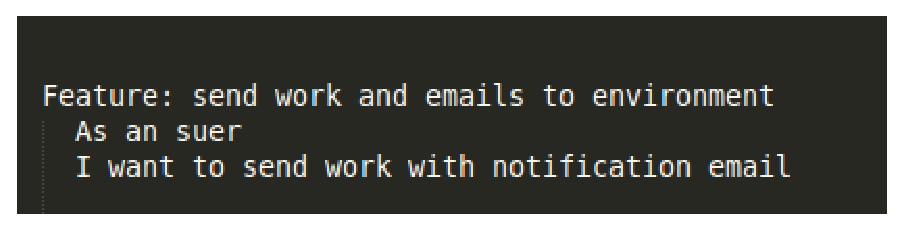
\includegraphics[keepaspectratio=true,scale=0.50]
      {figuras/noosfero_feature2.eps}
    \caption{Descrição do título (\textit{feature}) de um teste}
    \label{nosfero_feature}
\end{figure}

\item \textbf{Pré condições:} representado pela palavra-chave \textit{'background'}, define os passos 
precedem cada cenário de teste.

\begin{figure}[!h]
    \centering
    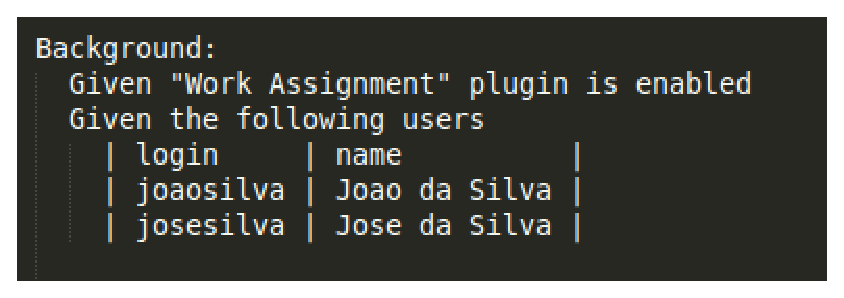
\includegraphics[keepaspectratio=true,scale=0.50]
      {figuras/noosfero_back.eps}
    \caption{Descrição de pré condições (\textit{background}) de um teste}
    \label{nosfero_feature}
\end{figure}

\item \textbf{Cenários:} representam parte concreta de como o software deve se 
comportar, e sendo a parte essencial do teste realizado no 
cucumber. Após a palavra-chave \textit{‘scenario’} define-se o nome do cenário em questão:
\item \textbf{Passos:} Cada cenario possui uma série de passos que demontram o seu 
comportamento, que são linhas simples iniciadas com as seguintes palavras-chaves: 
\textit{Given, When, Then, And, But}.
\item \textbf{Given:} Indica uma condição inicial para que o cenário seja executado, 
trata-se das pré-condições do cenário.
\item \textbf{When:} Indica o evento do cenário
\item \textbf{Then:} Indica o que é esperado após o evento ocorrer.

\begin{figure}[!h]
    \centering
    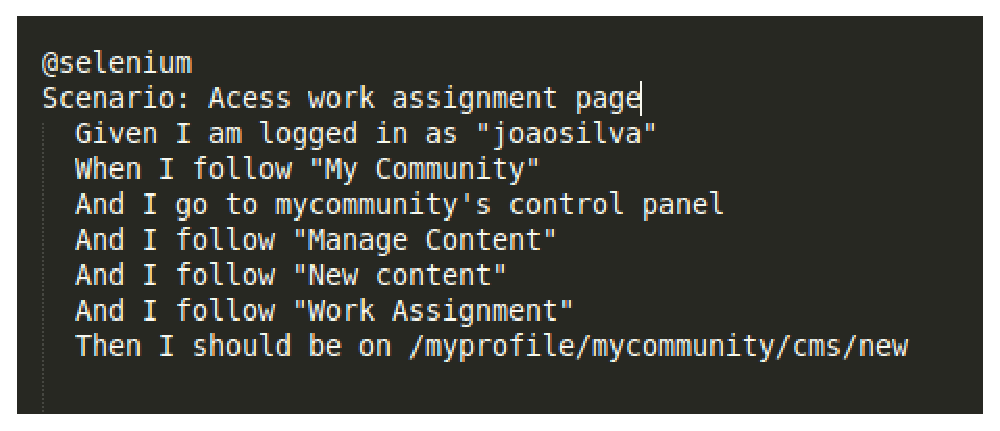
\includegraphics[keepaspectratio=true,scale=0.50]
      {figuras/noosfero_scenario.eps}
    \caption{Descrição do cenário (\textit{scenario}) de um teste}
    \label{nosfero_scenario}
\end{figure}

\end{enumerate}
Além do cucumber, também é utilizado um software chamado selenium, que é uma ferramenta
usada para desenvolver casos de testes a partir de \textit{web browsers}, como o mozilla firefox. Estas duas ferramentas, cucumber e selenium, utilizadas em conjunto, proporciona ao desenvolvedor a facilidade ao escrever os casos de testes em linguagem pura simular a execução automática destes testes em um \textit{web browser}. Porém o cucumber não faz tudo em linguagem pura, é necessário que outro código seja desenvolvido, em Ruby, fazendo par por baixo dos panos com a linguagem pura e executando os testes~\cite{akita2011}.

\subsection{Testes Funcionais e Unitários}
%
Os testes funcionais tem como objetivo no desenvolvimento na plataforma noosfero, verificara integraçao da aplicação desenvolvida. Os testes unitários são executados em conjunto com os testes funcionais, porém  com o objetivocde verificar trechos menores de códigos. Assim os testes funcionais e unitários são escritos da seguinte forma:

\textbf{Setup:} indica as condições inciais dos testes, setando variáveis de ambiente e de configuração por exemplo.

\begin{figure}[!h]
    \centering
    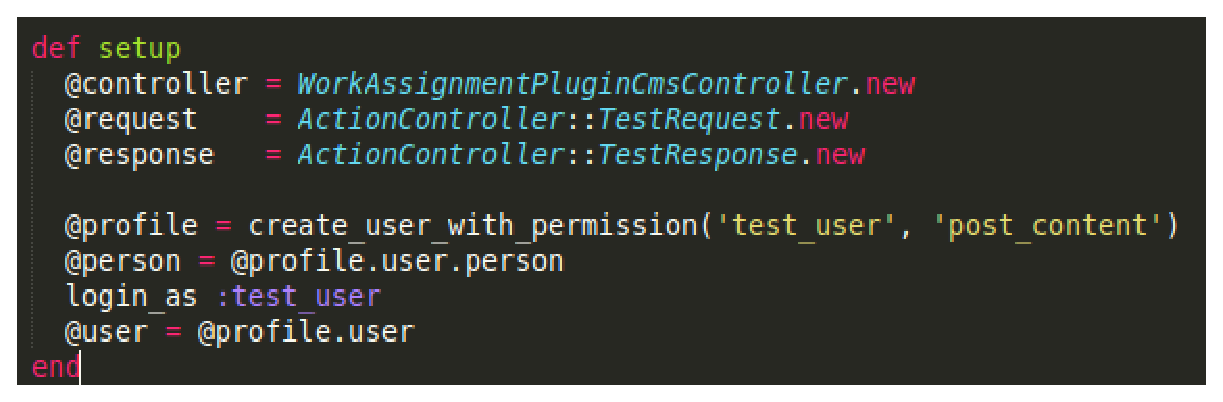
\includegraphics[keepaspectratio=true,scale=0.5]
      {figuras/teste_setup.eps}
    \caption{Descrição do setup de um teste}
    \label{nosfero_setup}
\end{figure}

\textbf{Título:} título do teste iniciado com a palavra \textit{‘should’} e finalizado com \textit{‘do’}

\textbf{Passos:} código que define o comportamento do teste

\textbf{Verificação:} Assertiva que verifica se a ação foi realizada como esperada.

\begin{figure}[!h]
    \centering
    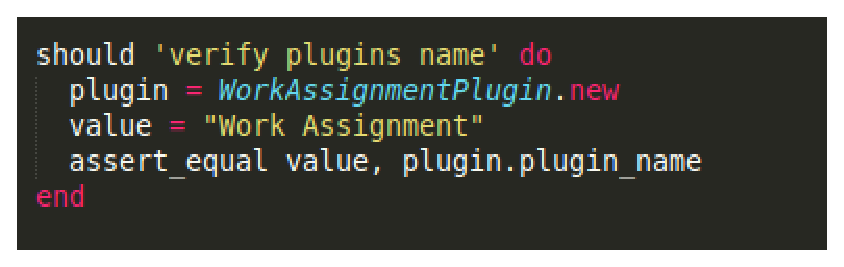
\includegraphics[keepaspectratio=true,scale=0.55]
      {figuras/teste_should.eps}
    \caption{Código de teste}
    \label{noosfero_should}
\end{figure}

\subsection{Plugin Ldap UnB}
%
Como rede colaborativa dos membros da Universidade de Brasília, o Comunidade UnB 
necessita possuir restrição de acesso aos usuários, para que somente membros ativos 
da universidade tenham acesso ao conteúdo da rede colaborativa. 
%
Para que esta necessidade fosse satisfeita foi desenvolvido um \textit{plugin} no noosfero, que efetuasse as restrições necessárias, utilizando o protocolo de autenticação da UnB, o LDAP.
%
\textit{Lightweight Directory Access Protocol} (LDAP) é um protocolo de aplicação 
aberto para acesso e manutenção  de serviços de informação de diretório distribuídos 
na internet~\cite{sermersheim2006}.
%
Os serviços de diretório desempenham um papel importante no desenvolvimento de aplicativos 
de intranet e internet, permitindo o compartilhamento de informações sobre os usuários, 
sistemas, redes, serviços e aplicações em toda a rede~\cite{oracle2000}.
%
Um cliente inicia uma sessão de LDAP através da ligação a um servidor LDAP, chamado 
\textit{Directory System Agent} (DSA), por padrão, a porta TCP e UDP porta 389. Após 
a conexão,é requerida ao servidor uma operação do cliente, e o servidor responde a 
mesma. 
%
Para o usuário, o \textit{plugin} desenvolvido modifica a seção de cadastro de novos usuários e a seção de \textit{login} de usuários. Na seção de cadastro o usuário agora deve cadastrar a matrícula e senha que o mesmo usa no matricula web da UnB\footnote{url{matriculaweb.unb.br}}, além dos dados que já eram cadastrados anteriormente. Na seção de \textit{login} o usuário também pode entrar no Comunidade UnB através de sua matrícula e senha do matrícula web da UnB (além do \textit{email} e \textit{username} 
- entradas normalmente utilizadas)
%
Nas camadas mais inferiores, o \textit{plugin} é responsável por modificar o modelo de dados do sistema, para que o usuário possa assim cadastrar sua matrícula. Assim o \textit{plugin} também é responsável por configurar a conexão com o LDAP server da UnB e finalmente verificar se os dados do usuário estão corretos no momento do seu cadastro. Abaixo encontra-se descritas as histórias de usuário referente ao {plugin} Ldap UnB:
\begin{enumerate}

\item \textbf{Plugin Ldap UnB - Cadastro:}

\textbf{Como} aluno da UnB e novo usuário

\textbf{Gostaria} de cadastra-me no Comunidade UnB através da minha matrícula e senha do sistemas da UnB

\textbf{para} utilizar o Comunidade UnB.

\textbf{Cenário:}

\textbf{Dado} que não estou autenticado

\textbf{Quando} eu entrar em ``Novo Usuário''

\textbf{E} preencher os campos ``nome de usuário'', ``senha'', ``confirmação de senha'', ``nome completo'', ``e-mail'' e ``matrícula''

\textbf{E} clicar no botão ``Registrar''

\textbf{Então} eu devo ser redirecionado ao perfil ``nome de usuário''


\item  \textbf{Plugin Ldap UnB - Login:}

\textbf{Como} aluno da UnB usuário do sistema

\textbf{Gostaria} acessar Comunidade UnB através da minha matrícula e senha do sistemas da UnB

\textbf{para} facilitar a utilização do Comunidade UnB.

\textbf{Cenário:}

\textbf{Dado} que não estou autenticado

\textbf{Quando} eu preencher os campos ``nome de usuário'' e ``senha''

\textbf{E} clicar em ``entrar''

\textbf{Então} eu devo ser redirecionado ao perfil ``nome de usuário''

\end{enumerate}

\subsubsection{Testes com \textit{plugin} LDAP}
%
Foram realizados os seguintes testes  com o plugin LDAP unb: testes funcionais e testes 
unitários. Os testes funcionais e unitários foram executados através 
do próprio noosfero, já os testes de aceitação foram executados com auxílio das ferramentas cucumber e selenium.
%
\subsubsection{Testes Funcionais}
%
Os testes funcionais do \textit{plugin} LDAP foram divididos em duas categorias, sendo estas compostas por testes que não dependem do LDAP está configurado e os testes que dependem do LDAP configurado. Os testes independentes do LDAP são simples, basicamente verificando as possíveis mensagem de errro ou de notificações durante o \textit{login}. Os testes  que dependem do LDAP verificam os seguintes fatores:
%
\begin{enumerate}
\item Autenticação de usuário com LDAP;
\item Autenticação de usuário a partir da sua matrícula;
\item Exibição de mensagens de logs
\item Criação de usuário utilizando as propriedades do LDAP;
\item Não autenticação de usuário registadro localmente, mas não com LDAP;
\item Não autenticação de usuário não registrado localmente, mas com LDAP;
\item Criação e autenticação de um novo usuário a partir do plugin LDAP;
\end{enumerate}
%
Também foram executados testes na interface de administrador do sistema, onde o usuário tem a opção de ativar o plugin e informar dados de configuração do mesmo, estes testes verificam os seguintes fatores:
%
\begin{enumerate}
\item Acesso à página de administrador;
\item Exibição de mensagens de sucesso e de erro;
\item Atualização do LDAP;
\item Atualização do host do LDAP;
\item Atualização da porta do LDAP;
\item Atualização da conta do LDAP;
\item Atualização da senha do LDAP;
\item Atualização da base dn;
\item Atualização do atributo de \textit{login};
\item Atualização do atributo de \textit{email};
\item Atualização do filtro do LDAP;
\item Atualização de TLS;
\end{enumerate}

% -------------PENSAR EM IMAGENS-----------------------%

\subsubsection{Testes unitários}
%
Os testes unitários do \textit{plugin} verificam a definição dos parâmetros do LDAP, verificação esta que é realizada tanto na passagem dos parâmentros quanto na verificação dos valores de \textit{default}, outra verificação destes parâmetros que também é feita é a tentativa de criação de uma autenticação no LDAP. Dentre estes parâmetros estão os seguintes:

\begin{itemize}
\item Host do LDAP;
\item Porta do LDAP;
\item Conta do LDAP;
\item Senha da conta;
\item Base DN do LDAP;
\item atributo de \textit{login} do LDAP;
\item atributo de nome do LDAP;
\item atributo de \textit{email} do LDAP;
\item filtros do LDAP;
\item TLS do LDAP;
\end{itemize}

Não foram desenvolvidos testes de aceitação para o \textit{plugin} LDAP Unb, pelo fato de ser uma aplicação que opera a maior parte das suas funcionalidades nas camadas mais baixas do sistema, alterando muito pouco a percepção do usuário.

\subsection{Plugin para submissão de trabalho}

Este \textit{plugin} também foi desenvolvido para a plataforma Noosfero, porém em uma aplicãção diferente, o Portal da FGA. A ideia deste \textit{plugin} surgiu da necessidade de existir um ambiente virtual em que os trabalhos de conclusão de curso pudessem ser submetidos aos professores e compartilhados com a comunidade acadêmica, buscando assim manter uma forma de versionamento dos trabalhos desenvolvidos.
%
Este \textit{plugin} é responsável por criar uma atribuição de trabalhos, chamada de \textit{work assignment}. Atribuição que possui algumas funcionalidades específicas como possibilitar que os usuários envolvidos sejam notificados via \textit{email} sobre a submissão de um certo trabalho. Para tal foi necessário subir um servidor de \textit{email} para executar estas notificações, assim como criar uma página no Portal FGA\footnote{url{www.fga.unb.br}} para que o usuário pudesse submeter seu trabalho.
%
O processo de desenvolvimento deste \textit{plugin} ocorreu juntamente com uma transição da equipe de desenvolvimento, o que prejudicou o desenvolvimento de testes do mesmo.
%
Para validar o desenvolvimento desta funcionalidade foram desenvolvidos os seguintes tipos de testes: funcionais, unitário e de aceitação. Abaixo encontra-se descrita a história de usuário referente \textit{plugin} submissão de trabalho:
\begin{enumerate}
\item  \textbf{Plugin submissão de trabalho}

\textbf{Como} usuário

\textbf{Gostaria} de submeter um trabalho para uma comunidade, seguindo um formulário (título, nome do remetente, \textit{email} do destinatário, nome do destinatário e descrição) enviando um aviso para ambas as partes

\textbf{para} manter um versionamento do trabalho.

x
\textbf{Cenário:}

\textbf{Dado} que estou autenticado como ``usuário''

\textbf{Quando} eu entrar no painel de controle da ``Minha Comunidade''

\textbf{E} entrar em ``Gerenciar Conteúdo''

\textbf{E} entrar em ``Novo Conteúdo''

\textbf{E} entrar em ``Trabalho a ser entregue''

\textbf{E} preencher o campo ``Título''

\textbf{E} clicar em ``Salvar''

\textbf{Então} eu devo ser redirecionado à pagina de ``Gerenciar Conteúdos''

\textbf{E} visualizar o campo ``Título''

\textbf{Quando} eu entrar em ``Carregar Arquivo''

\textbf{E} marcar o campo ``Enviar notificação''

\textbf{E} preencher o campo ``Assunto''

\textbf{E} preencher o campo ``Destinatário''

\textbf{E} clicar em ``Enviar''

\textbf{Então} eu devo visualizar ``Enviando com sucesso''

\end{enumerate}

\subsubsection{Testes Funcionais}

Os testes funcionais do \textit{plugin} para submissão de trabalho são responsáveis por verificar os seguintes fatores:

\begin{itemize}
\item Permissão para enviar trabalhos somente para usuários autorizados;
\item Capacidade de enviar um arquivo ou mais;
\item Capacidade de atualizar um arquivo enviado;
\item Validação de arquivos;
\item Capacidade de enviar \textit{email} aos usuários envolvidos;
\item Tratamento do redirecionamento das páginas;
\item Capacidade de deletar arquivos por usuários autorizados;
\item Capacidade de carregar arquivos por usuários envolvidos;
\end{itemize}

\subsubsection{Testes Unitários}

Os testes unitários do \textit{plugin} para submissão de trabalho são responsáveis por verificar os seguintes parâmetros:

\begin{itemize}
\item Nome do \textit{plugin};
\item Descrição do \textit{plugin};
\item Possibilidade de submissão de um arquivo por um usuário;
\item Nome do arquivo;
\item Versão do arquivo;
\item Autor do arquivo;
\end{itemize}

\subsubsection{Testes de Aceitação}

Os testes de aceitação do \textit{plugin} para submissão de trabalho são responsáveis por verificar os seguintes fatores:

\begin{itemize}
\item Capacidade de criar, editar e deletar uma atribuição de trabalhos (\textit{work assignment});
\item Validação de parâmetros durante a criação e edição de uma atribuição de trabalhos;
\item Capacidade de enviar e receber emails sobre o envio de um trabalho;
\item Capacidade de postar comentários sobre uma atribuição de trabalhos;
\item Capacidade de reportar problemas;
\end{itemize}

Abaixo estão descritos os testes desenvolvidos para o \textit{plugin}:


\textbf{Feature: send work plugin}

\textbf{As} an user

\textbf{I want} to send work with notification email

\textbf{Background:}

\textbf{Given} ``Work Assignment'' plugin is enabled

\textbf{Given} the following users

      | login     | name          |

      | joaosilva | Joao da Silva |

      | josesilva | Jose da Silva |

\textbf{And} the following community

      | identifier  | name         |

      | mycommunity | My Community |

\textbf{And} ``Joao da Silva" is admin of ``My Community"

\textbf{And} I am logged in as admin

\textbf{And} I go to /admin/plugins

\textbf{And} I check ``Work Assignment"

\textbf{And} I press ``Save changes"

\textbf{Then} I should see ``Plugins updated successfully." 



\begin{enumerate}
\item  \textbf{Scenario:} Upload a file to work assignment and send a email
    
    \textbf{Given} I am logged in as ``joaosilva" 
    
    \textbf{When} I follow ``My Community"
    
    \textbf{When} I go to mycommunity's control panel
    
    \textbf{And} I follow ``Manage Content"
    
    \textbf{And} I follow ``New content"
    
    \textbf{And} I follow ``Work Assignment"
    
    \textbf{Then} I should be on /myprofile/mycommunity/cms/new
    
    \textbf{When} I fill in ``Title" with ``test"
    
    \textbf{And} I press ``Save"
    
    \textbf{Then} I should be on /mycommunity/test
    
    \textbf{When} I follow ``Upload files"
    
    \textbf{And} I check ``Send notification"
    
    \textbf{And} I attach the file ``public/images/rails.png" to ``uploadedfiles"
    
    \textbf{And} I press ``Upload"
    
    \textbf{Then} I should be on /myprofile/mycommunity/cms/sendemail
    
    \textbf{When} I fill in ``Title" with ``Work"
    
    \textbf{And} I fill in ``Receiver" with ``josesilva@example.com"
    
    \textbf{And} I fill in ``Message" with ``test"
    
    \textbf{And} I press ``Send"
    
    \textbf{Then} I should see ``Contact sent successfully"

\item \textbf{Scenario:} Create a work assignment and continue edition

    \textbf{Given} I am logged in as ``joaosilva" 
    
    \textbf{When} I follow ``My Community"
    
    \textbf{When} I go to mycommunity's control panel
    
    \textbf{And} I follow ``Manage Content"
    
    \textbf{And} I follow ``New content"
    
    \textbf{And} I follow ``Work Assignment"

    \textbf{Then} I should be on /myprofile/mycommunity/cms/new
    
    \textbf{When} I fill in ``Title" with ``test"
    
    \textbf{And} I press ``Save and continue"
    
    \textbf{Then} I should be on /myprofile/mycommunity/cms/edit/13

 
\item \textbf{Scenario:} Can't create work assignment without name
    
    \textbf{Given}  I am logged in as ``joaosilva" 
    
    \textbf{When} I follow ``My Community"
    
    \textbf{When} I go to mycommunity's control panel
    
    \textbf{And} I follow ``Manage Content"
    
    \textbf{And} I follow ``New content"
    
    \textbf{And} I follow ``Work Assignment"
    
    \textbf{Then} I should be on /myprofile/mycommunity/cms/new
    
    \textbf{When} I fill in ``Title" with ``"
    
    \textbf{And} I press ``Save"
    
    \textbf{Then} I should see ``There were problems with the following fields:"

\item \textbf{Scenario:} Can't create work assignment without file
   
    \textbf{Given} I am logged in as ``joaosilva" 
   
    \textbf{When} I follow ``My Community"
   
    \textbf{When} I go to mycommunity's control panel
   
    \textbf{And} I follow ``Manage Content"
   
    \textbf{And} I follow ``New content"
   
    \textbf{And} I follow ``Work Assignment"
   
    \textbf{Then} I should be on /myprofile/mycommunity/cms/new
   
    \textbf{When} I fill in ``Title" with ``test"
   
    \textbf{And} I press ``Save"
   
    \textbf{Then} I should be on /mycommunity/test
   
    \textbf{When} I follow ``Upload files"
   
    \textbf{And} I press ``Upload"
   
    \textbf{Then} I should be on /myprofile/mycommunity/cms/uploadfiles

\item \textbf{Scenario:} Cancel create work assignment
    
    \textbf{Given} I am logged in as ``joaosilva"
    
    \textbf{When} I follow ``My Community"
    
    \textbf{When} I go to mycommunity's control panel
    
    \textbf{And}  I follow ``Manage Content"
    
    \textbf{And}  I follow ``New content"
    
    \textbf{And}  I follow ``Work Assignment"
    
    \textbf{Then} I should be on /myprofile/mycommunity/cms/new
    
    \textbf{When} I fill in ``Title" with ``test"
    
    \textbf{And}  I press ``Save"
    
    \textbf{Then} I should be on /mycommunity/test
    
    \textbf{When} I follow ``Upload files"
    
    \textbf{And}  I follow ``Cancel"
    
    \textbf{Then} I should be on /mycommunity/test

\item \textbf{Scenario:} Edit work assignment 
    
    \textbf{Given} I am logged in as ``joaosilva"
    
    \textbf{When} I follow ``My Community"
    
    \textbf{When} I go to mycommunity's control panel
    
    \textbf{And} I follow ``Manage Content"
    
    \textbf{And} I follow ``New content"
    
    \textbf{And} I follow ``Work Assignment"
    
    \textbf{Then} I should be on /myprofile/mycommunity/cms/new
    
    \textbf{When} I fill in ``Title" with ``test"
    
    \textbf{And} I press ``Save"
    
    \textbf{Then} I should be on /mycommunity/test
    
    \textbf{When} I follow ``Edit"
    
    \textbf{And} I fill in ``Title" with ``test2"
    
    \textbf{And} I press ``Save"
    
    \textbf{Then} I should be on /mycommunity/test2

\item \textbf{Scenario:} Delete a work assignment  
   
    \textbf{Given} I am logged in as ``joaosilva"
   
    \textbf{When} I follow ``My Community"
   
    \textbf{When} I go to mycommunity's control panel
   
    \textbf{And} I follow ``Manage Content"
   
    \textbf{And} I follow ``New content"
   
    \textbf{And} I follow ``Work Assignment"
   
    \textbf{Then} I should be on /myprofile/mycommunity/cms/new
   
    \textbf{When} I fill in ``Title" with ``test"
   
    \textbf{And} I press ``Save"
   
    \textbf{Then} I should be on /mycommunity/test
   
    \textbf{When} I follow ``Edit"
   
    \textbf{And} I follow ``Delete"
   
    \textbf{And} I confirm the browser dialog
   
    \textbf{Then} I should see /``test" was removed./
    
\end{enumerate}

\section{Considerações finais}

O desenvolvimento de testes automatizados é uma prática constante no desenvolvimento da plataforma noosfero e importante na validação de novos recursos desenvolvidos. Assim conseguimos verificar que a utilização de práticas de TDD e BDD como base para o desenvolvimento trouxe resultados satisfatórios, como será mostrado no capítulo a seguir.
